\documentclass{beamer}
\usepackage[utf8]{inputenc}
\usetheme{Madrid}
\usecolortheme{default}
\usepackage{amsmath,amssymb,amsfonts,amsthm}
\usepackage{txfonts}
\usepackage{tkz-euclide}
\usepackage{listings}
\usepackage{adjustbox}
\usepackage{array}
\usepackage{tabularx}
\usepackage{gvv}
\usepackage{lmodern}
\usepackage{circuitikz}
\usepackage{tikz}
\usepackage{graphicx}
\setbeamertemplate{page number in head/foot}[totalframenumber]
\usepackage{tcolorbox}
\tcbuselibrary{minted,breakable,xparse,skins}
\definecolor{bg}{gray}{0.95}
\DeclareTCBListing{mintedbox}{O{}m!O{}}{%
  breakable=true,
  listing engine=minted,
  listing only,
  minted language=#2,
  minted style=default,
  minted options={%
    linenos,
    gobble=0,
    breaklines=true,
    breakafter=,,
    fontsize=\small,
    numbersep=8pt,
    #1},
  boxsep=0pt,
  left skip=0pt,
  right skip=0pt,
  left=25pt,
  right=0pt,
  top=3pt,
  bottom=3pt,
  arc=5pt,
  leftrule=0pt,
  rightrule=0pt,
  bottomrule=2pt,
  toprule=2pt,
  colback=bg,
  colframe=orange!70,
  enhanced,
  overlay={%
    \begin{tcbclipinterior}
    \fill[orange!20!white] (frame.south west) rectangle ([xshift=20pt]frame.north west);
    \end{tcbclipinterior}},
  #3,
}
\lstset{
    language=C,
    basicstyle=\ttfamily\small,
    keywordstyle=\color{blue},
    stringstyle=\color{orange},
    commentstyle=\color{green!60!black},
    numbers=left,
    numberstyle=\tiny\color{gray},
    breaklines=true,
    showstringspaces=false,
}
\begin{document}
\title 
{5.2.62}
\date{september 2025}
\author 
{Namaswi-EE25BTECH11060}
\frame{\titlepage}
\begin{frame}{Question}Solve system of linear equations \\
\begin{align*}
3x-2y+3z=8\\2x+y-z=1\\4x-3y+2z=4
\end{align*}
\end{frame}
\begin{frame}{Solution}
According to question the Equations of line given are\\
\begin{align}
\begin{pmatrix}
  3 & -2 & 3  
\end{pmatrix}X=8\\
\begin{pmatrix}
   2 & 1 & -2  
\end{pmatrix}X=1\\
\begin{pmatrix}
 4 & -3 & 2   
\end{pmatrix}X=4\\
\begin{pmatrix}
    3 & -2 & 3 \\
    2 & 1 & -1\\
    4 & -3 & 2
\end{pmatrix}X=\begin{pmatrix}
    8 \\ 1\\ 4
\end{pmatrix}
\end{align}    
\end{frame}
\begin{frame}{Solution}
    Forming Argumented Matrix\\
\begin{align}
\left(\begin{array}{ccc|c}
3 & -2 & 3 & 8 \\[4pt]
2 & 1 & -1 & 1 \\[4pt]
4 & -3 & 2 & 4
\end{array}\right).
\end{align}
Replace
 \[
R_1 \to \tfrac{1}{3}R_3
\]
\begin{align}
\augvec{3}{1}{
1 & -\frac{2}{3} & 1 &  \frac{8}{3} \\
2 & 1 & -1 & 1 \\
4 & -3 & 2 & 4}
\end{align}
\end{frame}
\begin{frame}{Solution}
 Replace
\[
R_2 \to R_2 - 2R_1, 
\quad
R_3 \to R_3 - 4R_1
\]
\begin{align}
\augvec{3}{1}{
1 & -\tfrac{2}{3} & 1 & \tfrac{8}{3} \\
0 & \tfrac{7}{3} & -3 & -\tfrac{13}{3} \\
0 & -\tfrac{1}{3} & -2 & -\tfrac{20}{3}
        }
\end{align}
Replace
\[
R_2 \to \tfrac{3}{7}R_2
\]
\begin{align}
  \augvec{3}{1}{
1 & -\tfrac{2}{3} & 1 & \tfrac{8}{3} \\
0 & 1 & -\tfrac{9}{7} & -\tfrac{13}{7} \\
0 & -\tfrac{1}{3} & -2 & -\tfrac{20}{3}
 }  
\end{align}   
\end{frame}
\begin{frame}{Solution}
    Replace
\[
R_1 \to R_1 + \tfrac{2}{3}R_2, 
\quad
R_3 \to R_3 + \tfrac{1}{3}R_2
\]

\begin{align}
\augvec{3}{1}{ 
1 & 0 & \tfrac{5}{21} & \tfrac{22}{21} \\
0 & 1 & -\tfrac{9}{7} & -\tfrac{13}{7} \\
0 & 0 & -\tfrac{41}{21} & -\tfrac{143}{21}}
\end{align}
Replace
\[
R_3 \to -\tfrac{21}{41}R_3
\]
\begin{align}
\augvec{3}{1}{ 1 & 0 & \tfrac{5}{21} & \tfrac{22}{21} \\
0 & 1 & -\tfrac{9}{7} & -\tfrac{13}{7} \\ 
0 & 0 & 1 & \tfrac{143}{41} }
\end{align}
\end{frame}
\begin{frame}{Solution}
    Replace
\[
R_1 \to R_1 - \tfrac{5}{21}R_3, 
\quad
R_2 \to R_2 + \tfrac{9}{7}R_3
\]
 \begin{align}
\augvec{3}{1}{1 & 0 & 0 & \tfrac{62}{123} \\
0 & 1 & 0 & \tfrac{110}{287} \\
0 & 0 & 1 & \tfrac{143}{41}}   
\end{align}
Hence,
\begin{align}
\Vec{X}=\begin{pmatrix}
\tfrac{62}{123}\\ 
 \tfrac{110}{287} \\
 \tfrac{143}{41}
\end{pmatrix}
\end{align}
\end{frame}
\begin{frame}[fragile]
\frametitle{C Code}
\begin{lstlisting}
   #include <stdio.h>
int main() {
    int n = 3;
    double a[3][4] = {
        {3, -2, 3, 8},
        {2, 1, -1, 1},
        {4, -3, 2, 4}
    };
    // Forward elimination
    for (int i = 0; i < n; i++) {
        // Normalize row
        double pivot = a[i][i];
        for (int j = i; j <= n; j++)
            a[i][j] /= pivot; 
\end{lstlisting}
\end{frame}
\begin{frame}[fragile]
\frametitle{C Code}
\begin{lstlisting}
     // Eliminate column
        for (int k = 0; k < n; k++) {
            if (k != i) {
                double factor = a[k][i];
                for (int j = i; j <= n; j++)
                    a[k][j] -= factor * a[i][j];
            }
        }
    }

    printf("Solution:\n");
    for (int i = 0; i < n; i++) {
        printf("x%d = %lf\n", i+1, a[i][n]);
    }

    return 0;
}
\end{lstlisting}
\end{frame}
\begin{frame}[fragile]
\frametitle{Python Code}
\begin{lstlisting}
    import numpy as np
import matplotlib.pyplot as plt
from mpl_toolkits.mplot3d import Axes3D   # registers 3D projection
from matplotlib.patches import Patch

# Plane coefficients: a*x + b*y + c*z = d
planes = [
    (3, -2,  3, 8,  "3x - 2y + 3z = 8"),
    (2,  1, -1, 1,  "2x +  y -  z = 1"),
    (4, -3,  2, 4,  "4x - 3y + 2z = 4")
]
colors = ["tab:blue", "tab:orange", "tab:green"]

# Solve linear system to find intersection point (if unique)
A = np.array([[p[0], p[1], p[2]] for p in planes], dtype=float)
b = np.array([p[3] for p in planes], dtype=float)
\end{lstlisting}
\end{frame}
\begin{frame}[fragile]
\frametitle{Python Code}
\begin{lstlisting}
    intersection = None
try:
    intersection = np.linalg.solve(A, b)   # [x0, y0, z0]
    has_unique = True
except np.linalg.LinAlgError:
    has_unique = False

# Build a grid in x-y around the intersection (or default range)
if has_unique:
    x0, y0, z0 = intersection
    rng = 3.0
    x_min, x_max = x0 - rng, x0 + rng
    y_min, y_max = y0 - rng, y0 + rng
else:
    x_min, x_max = -5, 5
    y_min, y_max = -5, 5
\end{lstlisting}
\end{frame}
\begin{frame}[fragile]
    \frametitle{Python Code}
    \begin{lstlisting}
        xx, yy = np.meshgrid(np.linspace(x_min, x_max, 40),
                     np.linspace(y_min, y_max, 40))

fig = plt.figure(figsize=(10, 8))
ax = fig.add_subplot(111, projection='3d')

# Plot each plane
patches = []
for (a, b_coef, c, d, label), col in zip(planes, colors):
    # compute z = (d - a*x - b*y)/c  (works since c != 0 for these planes)
    zz = (d - a * xx - b_coef * yy) / c
    surf = ax.plot_surface(xx, yy, zz, alpha=0.5, rstride=1, cstride=1, linewidth=0, antialiased=True)
    patches.append(Patch(facecolor=col, label=label))
    # Color the surface by setting the facecolors (plot_surface doesn't accept label directly)
    surf.set_facecolor(col)
    surf.set_edgecolor((0,0,0,0))  # hide edges for smooth look
    \end{lstlisting}
\end{frame}
\begin{frame}[fragile]
    \frametitle{Python Code}
    \begin{lstlisting}
        # Plot intersection point if exists
if has_unique:
    ax.scatter([x0], [y0], [z0], color="red", s=60, label="Intersection point")
    ax.text(x0, y0, z0, f"  ({x0:.2f}, {y0:.2f}, {z0:.2f})", color="red")

# Labels, limits and legend
ax.set_xlabel("X")
ax.set_ylabel("Y")
ax.set_zlabel("Z")
ax.set_xlim(x_min, x_max)
ax.set_ylim(y_min, y_max)
    \end{lstlisting}
\end{frame}
\begin{frame}[fragile]
    \frametitle{Python Code}
    \begin{lstlisting}
     # Create legend: include plane labels and intersection point if present
legend_handles = [Patch(facecolor=colors[i], label=planes[i][4]) for i in range(len(planes))]
if has_unique:
    legend_handles.append(plt.Line2D([0], [0], marker='o', color='w',
                                     markerfacecolor='red', markersize=8, label='Intersection point'))
ax.legend(handles=legend_handles, loc='upper left', bbox_to_anchor=(1.05, 1))

ax.set_title("3 Planes: 3x-2y+3z=8, 2x+y-z=1, 4x-3y+2z=4")
plt.tight_layout()
plt.show()   
    \end{lstlisting}
\end{frame}
\begin{frame}[fragile]
    \frametitle{C and Python Code}
    \begin{lstlisting}
       import ctypes
import numpy as np
# Load the shared library
gauss = ctypes.CDLL("./gauss.so")
# Define argument types
gauss.gauss.argtypes = [((ctypes.c_double * 4) * 3), ctypes.POINTER(ctypes.c_double)]
# Input augmented matrix
A = np.array([
    [3, -2, 3, 8],
    [2,  1, -1, 1],
    [4, -3, 2, 4]
], dtype=np.float64)
 
    \end{lstlisting}
\end{frame}
\begin{frame}[fragile]
    \frametitle{C and Python Code}
    \begin{lstlisting}
        # Convert numpy to C array
a_c = ((ctypes.c_double * 4) * 3)(*([tuple(row) for row in A]))

# Allocate solution vector
sol = (ctypes.c_double * 3)()

# Call C function
gauss.gauss(a_c, sol)

# Print solution
print("Solution from C function:")
print("x =", sol[0])
print("y =", sol[1])
print("z =", sol[2])
    \end{lstlisting}
\end{frame}
\begin{frame}{plot}
     \centering
    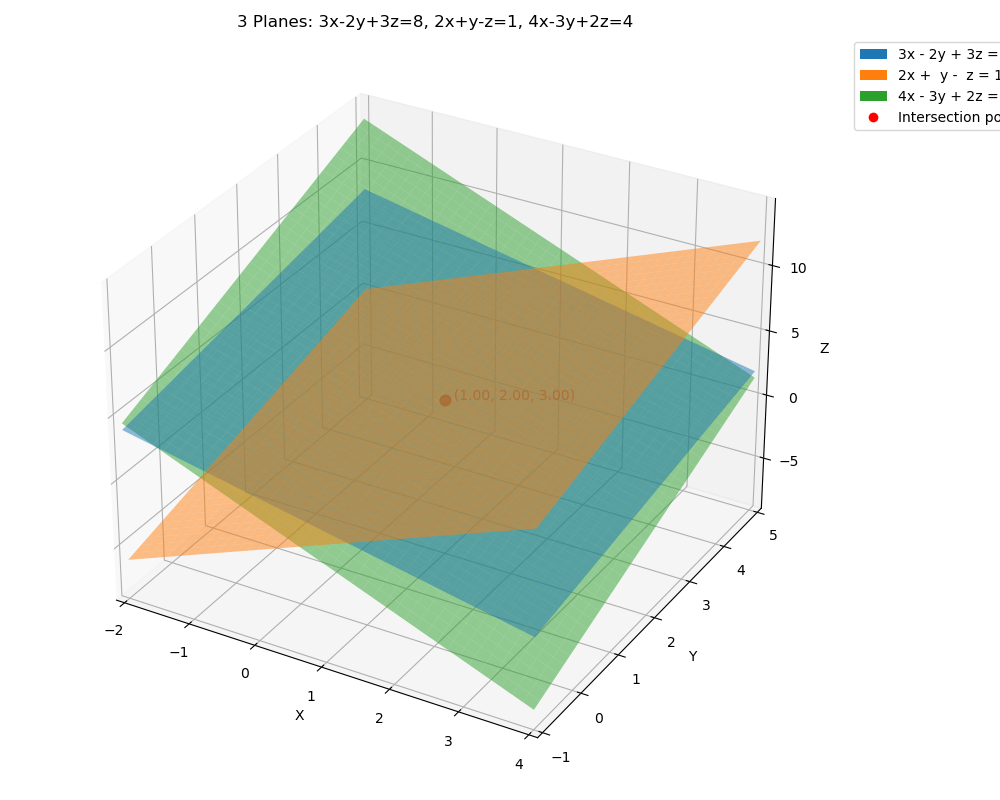
\includegraphics[width=\columnwidth, height=0.8\textheight, keepaspectratio]{Figure_10.png} 
\end{frame}
\end{document}